\documentclass[journal,12pt,twocolumn]{IEEEtran}

\usepackage{setspace}
\usepackage{gensymb}
\singlespacing
\usepackage[cmex10]{amsmath}

\usepackage{amsthm}

\usepackage{mathrsfs}
\usepackage{txfonts}
\usepackage{stfloats}
\usepackage{bm}
\usepackage{cite}
\usepackage{cases}
\usepackage{subfig}

\usepackage{longtable}
\usepackage{multirow}

\usepackage{enumitem}
\usepackage{mathtools}
\usepackage{steinmetz}
\usepackage{tikz}
\usepackage{circuitikz}
\usepackage{verbatim}
\usepackage{tfrupee}
\usepackage[breaklinks=true]{hyperref}
\usepackage{graphicx}
\usepackage{tkz-euclide}

\usetikzlibrary{calc,math}
\usepackage{listings}
    \usepackage{color}                                            %%
    \usepackage{array}                                            %%
    \usepackage{longtable}                                        %%
    \usepackage{calc}                                             %%
    \usepackage{multirow}                                         %%
    \usepackage{hhline}                                           %%
    \usepackage{ifthen}                                           %%
    \usepackage{lscape}     
\usepackage{multicol}
\usepackage{chngcntr}

\DeclareMathOperator*{\Res}{Res}

\renewcommand\thesection{\arabic{section}}
\renewcommand\thesubsection{\thesection.\arabic{subsection}}
\renewcommand\thesubsubsection{\thesubsection.\arabic{subsubsection}}

\renewcommand\thesectiondis{\arabic{section}}
\renewcommand\thesubsectiondis{\thesectiondis.\arabic{subsection}}
\renewcommand\thesubsubsectiondis{\thesubsectiondis.\arabic{subsubsection}}


\hyphenation{op-tical net-works semi-conduc-tor}
\def\inputGnumericTable{}                                 %%

\newcommand{\permcomb}[4][0mu]{{{}^{#3}\mkern#1#2_{#4}}}
\newcommand{\perm}[1][-3mu]{\permcomb[#1]{P}}
\newcommand*{\comb}[1][-1mu]{\permcomb[#1]{C}}

\lstset{
%language=C,
frame=single, 
breaklines=true,
columns=fullflexible
}
\begin{document}

\newcommand{\BEQA}{\begin{eqnarray}}
\newcommand{\EEQA}{\end{eqnarray}}
\newcommand{\define}{\stackrel{\triangle}{=}}
\bibliographystyle{IEEEtran}
\raggedbottom
\setlength{\parindent}{0pt}
\providecommand{\mbf}{\mathbf}
\providecommand{\pr}[1]{\ensuremath{\Pr\left(#1\right)}}
\providecommand{\qfunc}[1]{\ensuremath{Q\left(#1\right)}}
\providecommand{\sbrak}[1]{\ensuremath{{}\left[#1\right]}}
\providecommand{\lsbrak}[1]{\ensuremath{{}\left[#1\right.}}
\providecommand{\rsbrak}[1]{\ensuremath{{}\left.#1\right]}}
\providecommand{\brak}[1]{\ensuremath{\left(#1\right)}}
\providecommand{\lbrak}[1]{\ensuremath{\left(#1\right.}}
\providecommand{\rbrak}[1]{\ensuremath{\left.#1\right)}}
\providecommand{\cbrak}[1]{\ensuremath{\left\{#1\right\}}}
\providecommand{\lcbrak}[1]{\ensuremath{\left\{#1\right.}}
\providecommand{\rcbrak}[1]{\ensuremath{\left.#1\right\}}}
\theoremstyle{remark}
\newtheorem{rem}{Remark}
\newcommand{\sgn}{\mathop{\mathrm{sgn}}}
\providecommand{\abs}[1]{\vert#1\vert}
\providecommand{\res}[1]{\Res\displaylimits_{#1}} 
\providecommand{\norm}[1]{\lVert#1\rVert}
%\providecommand{\norm}[1]{\lVert#1\rVert}
\providecommand{\mtx}[1]{\mathbf{#1}}
\providecommand{\mean}[1]{E[ #1 ]}
\providecommand{\fourier}{\overset{\mathcal{F}}{ \rightleftharpoons}}
%\providecommand{\hilbert}{\overset{\mathcal{H}}{ \rightleftharpoons}}
\providecommand{\system}{\overset{\mathcal{H}}{ \longleftrightarrow}}
	%\newcommand{\solution}[2]{\textbf{Solution:}{#1}}
\newcommand{\solution}{\noindent \textbf{Solution: }}
\newcommand{\cosec}{\,\text{cosec}\,}
\providecommand{\dec}[2]{\ensuremath{\overset{#1}{\underset{#2}{\gtrless}}}}
\newcommand{\myvec}[1]{\ensuremath{\begin{pmatrix}#1\end{pmatrix}}}
\newcommand{\mydet}[1]{\ensuremath{\begin{vmatrix}#1\end{vmatrix}}}
\numberwithin{equation}{subsection}
\makeatletter
\@addtoreset{figure}{problem}
\makeatother
\let\StandardTheFigure\thefigure
\let\vec\mathbf
\renewcommand{\thefigure}{\theproblem}
\def\putbox#1#2#3{\makebox[0in][l]{\makebox[#1][l]{}\raisebox{\baselineskip}[0in][0in]{\raisebox{#2}[0in][0in]{#3}}}}
     \def\rightbox#1{\makebox[0in][r]{#1}}
     \def\centbox#1{\makebox[0in]{#1}}
     \def\topbox#1{\raisebox{-\baselineskip}[0in][0in]{#1}}
     \def\midbox#1{\raisebox{-0.5\baselineskip}[0in][0in]{#1}}
\vspace{3cm}
\title{AI1103 - Assignment 5}
\author{Aman Panwar - CS20BTECH11004}
\maketitle
\newpage
\bigskip
\renewcommand{\thefigure}{\theenumi}
\renewcommand{\thetable}{\theenumi}
%
Latex codes : 
%
\begin{lstlisting}
https://github.com/CS20BTECH11004/AI1103/blob/main/Assignment%205/Assignment%205.tex
\end{lstlisting}

\section*{Question: UGC/MATH (mathA\_June 2017), Q.118}
Suppose the random variable X has the following probability density funtion 
\begin{align}
    f(x)=\begin{cases}\alpha\brak{x-\mu}^{\alpha -1}e^{-\brak{x-\mu}^\alpha};&x>\mu\\
                        0                               &x\leq\mu    
    \end{cases}\nonumber
\end{align}
where $\alpha>0,-\infty <\mu<\infty$. Which of the following are correct? The hazard function of $X$ is
\begin{enumerate}
    \item an increasing function for all $\alpha>0$
    \item a decreasing function for all $\alpha >0$
    \item an increasing function for some $\alpha>0$
    \item a decreasing function for some $\alpha>0$
\end{enumerate}
\section*{Solution}
\newcommand{\Integral}[2]{\ensuremath{\int\limits_{#1}^{#2}}}
For the random variable $X$, the CDF is
\begin{align}
    F(x)&=\Integral{0}{x}f(y)dy\\
        &=\Integral{0}{\mu}0 dy +\Integral{\mu}{x}\alpha\brak{y-\mu}^{\alpha -1}e^{-\brak{y-\mu}^\alpha}\\
        &=0 -e^{-\brak{y-\mu}^\alpha}\Big|_{\mu}^{x}\\
        &=1-e^{-\brak{x-\mu}^{\alpha}}
\end{align}
For X, the hazard function $H(y)$ is defined as
\begin{align}
    H(y)&=\frac{f(y)}{1-F(y)}\nonumber\\
    \implies H(y)&=\begin{cases}\frac{\alpha\brak{y-\mu}^{\alpha -1}e^{-\brak{y-\mu}^\alpha}}{1-\brak{1-e^{-\brak{y-\mu}^{\alpha}}}};&y>\mu\\
                        0                               &y\leq\mu   
    \end{cases}\nonumber\\
    &=\begin{cases}\alpha\brak{y-\mu}^{\alpha -1};&y>\mu\\
                        0                            &y\leq\mu   
    \end{cases}\nonumber
\end{align}
Differentiating $H(y)$ w.r.t. $y$
\begin{align}
    H'(y)&=\begin{cases}\alpha\brak{\alpha - 1}\brak{y-\mu}^{\alpha -2};&y>\mu\\
                        0                            &y\leq\mu   
    \end{cases}\nonumber
\end{align}
When $y\leq \mu$ then $H'(y)$ is $0$. When $y>\mu$ then $\brak{y-\mu}^{\alpha -2}$ is positive. This implies that the sign for $H'(y)$ for $y>\mu$ is decided by the sign of $\alpha\brak{\alpha -1}$.
\begin{align}
    \alpha\brak{1-\alpha}<0
    \implies 0<\alpha<1\nonumber\\
    \alpha\brak{1-\alpha}>0\implies \alpha>1 &&\text{(ignoring $\alpha<0$)}\nonumber
\end{align}
$\therefore$ The Hazard function of $X$ is decreasing when $\alpha \in \brak{0,1}$ and increasing when $\alpha \in \brak{1,\infty}$


\vspace{0.5cm}\centering \boxed{\solution{\text{Options 3, 4}}}

\iffalse
\begin{figure}[h!]
    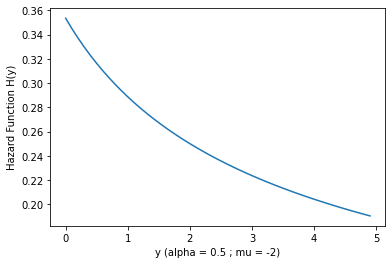
\includegraphics[width = \columnwidth]{Figure-1.png}
    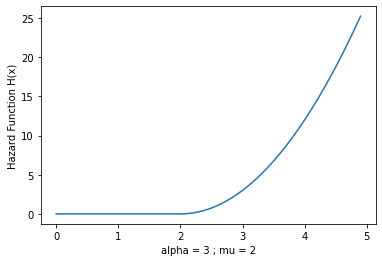
\includegraphics[width = \columnwidth]{Figure-2.png}
\end{figure}
\fi
\begin{figure}[h]
    \centering
    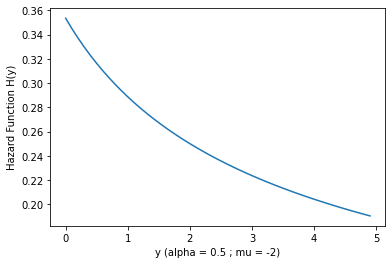
\includegraphics[width=\columnwidth-50pt]{Figure-1.png}
    \caption{Decreasing Hazard Function}
    \label{fig:my_label1}
\end{figure}
\begin{figure}[h]
    \centering
    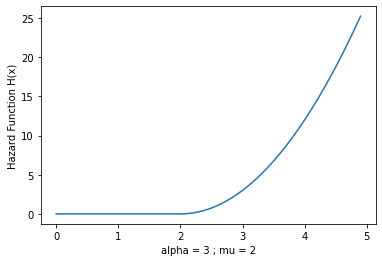
\includegraphics[width=\columnwidth-50pt]{Figure-2.png}
    \caption{Increasing Hazard Function}
    \label{fig:my_label2}
\end{figure}



\end{document}
